\section{Experiment results}

\subsection{Distribution of pull requests by size in sets}
To validate the statistical significance of our experiment, we examined the distribution of pull requests by size across all sets. Our analysis revealed a uniform distribution, lending credence to the robustness of our experimental design and the validity of our findings. This uniformity in size distribution across sets strengthens the reliability of our statistical inferences and the overall significance of the observed results. Refer to Figure \ref{fig:pr_dist_across_sets}.

\begin{figure}[htbp]
    \centering
    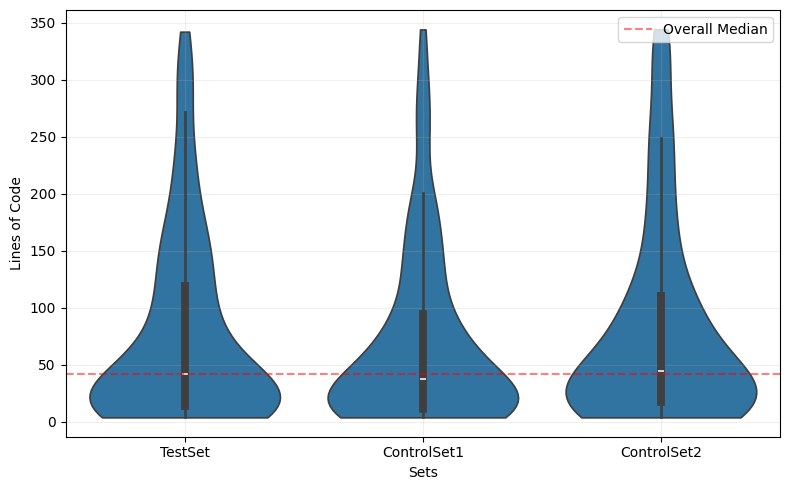
\includegraphics[width=1\columnwidth]
    {Figures/pr_dist.png}
    \caption{Distribution of PRs by sizes across sets. We can observe all 3 sets are similar}
    \label{fig:pr_dist_across_sets}
\end{figure}


\begin{figure*}[htbp]
    \centering
    \begin{subfigure}[t]{\columnwidth}
        \centering
        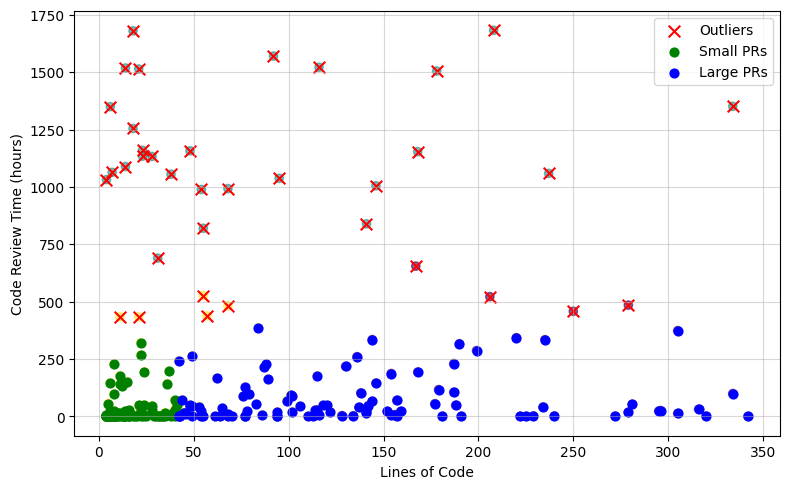
\includegraphics[scale=0.35]{Figures/test_dist.png}
        \caption{Test set with correlation coefficient of 0.095}
    \end{subfigure}%
    ~ 
    \begin{subfigure}[t]{\columnwidth}
        \centering
        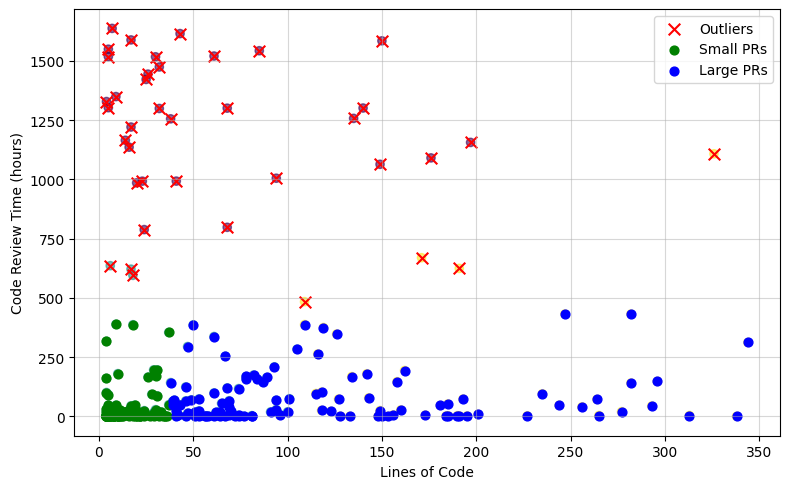
\includegraphics[scale=0.35]{Figures/control1_dist.png}
        \caption{Control 1 set with correlation coefficient of 0.004}
    \end{subfigure}

    \centering
    \begin{subfigure}[t]{\columnwidth}
        \centering
        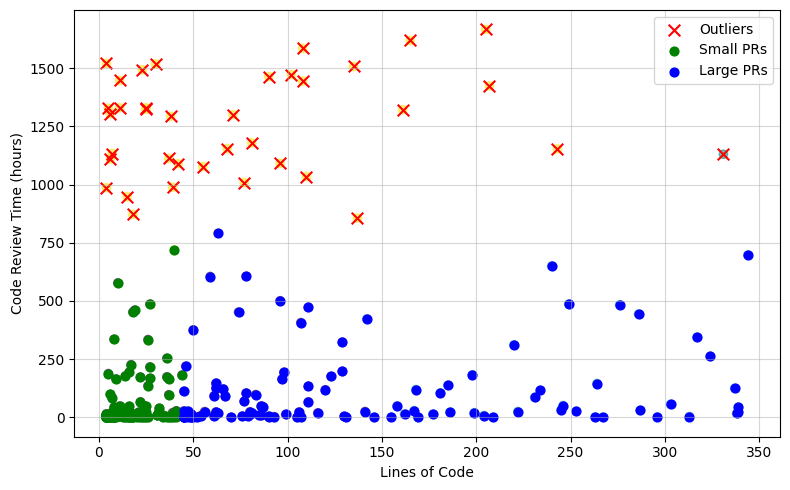
\includegraphics[scale=0.35]{Figures/control2_dist.png}
        \caption{Control 2 set with correlation coefficient of 0.052}
    \end{subfigure}%

    \caption{Weak correlation between lines of code changed in a pull request vs time to review that PR}
\label{fig:loc_vs_review_time_distribution}    
\end{figure*}

\subsection{Weak correlation between lines of code and code review time}
While one might expect a strong positive correlation between the number of lines of code to be reviewed and the time required for review, empirical evidence suggests otherwise. Contrary to intuition, experienced professionals in the field often observe a weak relationship between these variables. Our experimental results corroborate this phenomenon. As illustrated in Figure \ref{fig:loc_vs_review_time_distribution}, the correlation coefficients between lines of code changed and code review time for pull requests are notably low: 0.095, 0.004, and 0.052 for the test, control 1, and control 2 sets, respectively. These findings indicate a minimal association between the volume of code changes and the duration of the review process.

\subsection{Time savings due to DeputyDev intervention}
Our analysis extended to examining the average code review time per pull request (PR), per line of code, and the median code review time. The results revealed a statistically significant reduction in all these temporal metrics, primarily attributable to DeputyDev's interventions. This observation substantiates the hypothesis that DeputyDev's involvement in PR reviews leads to expedited turnaround times. A key factor contributing to this efficiency is the immediate feedback provided to PR authors upon submission, eliminating the delay typically associated with waiting for a human reviewer to initiate the review process. This immediate engagement appears to streamline the overall review workflow. Refer to Table \ref{tab:pr_review_stats} for numbers and Appendix \ref{app:calculations} for calculations.

\begin{table*}[ht]
\centering
\begin{tabularx}{\textwidth}{@{}l*{7}{>{\centering\arraybackslash}X}@{}}
\toprule
\hline
\textbf{Set} & \textbf{No. of PRs} & \textbf{Avg Loc Per PR} & \textbf{Avg Review Time (hrs)} & \textbf{Avg Review Time Per LOC (hrs)} & \textbf{Median Review Time (hrs)} \\
\hline
ControlSet1 (CS1) & 244 & 69 & 239.57 & 12.97 & 0.76 \\
ControlSet2 (CS2) & 238 & 82 & 278.14 & 12.29 & 0.78 \\
TestSet (TS) & 239 & 78 & 197.97 & 7.50 & 0.41 \\
\hline
\textbf{TS $\Delta$ CS1 (\%)} & - & - & -17.36 & -42.19 & -46.36\\
\textbf{TS $\Delta$ CS2 (\%)} & - & - & -28.82 & -38.98 & -47.52\\
\hline
\end{tabularx}
\caption{We observe significant decrease in avg review time, avg review time per LOC and median review time in Test set upto 28.82\%, 42.19\% and 47.52\% respectively}
\label{tab:pr_review_stats}
\end{table*}

\begin{table*}[ht]
\centering
\begin{tabularx}{\textwidth}{@{}l*{6}{>{\centering\arraybackslash}X}@{}}
\toprule
\hline
\textbf{PR size category(LOC)} & 
\textbf{CS1} & 
\textbf{CS2} & 
\textbf{TS} & 
\textbf{TS $\Delta$ CS1 (\%)} & 
\textbf{TS $\Delta$ CS2 (\%)} & 
\textbf{PR Count} \\
\hline
0-50 (S) & 21.23 & 20.34 & 11.92 & -43.87 & -41.40 & 399 \\
\hline
51-100 (M) & 2.61 & 4.09 & 3.50 & 34.01 & -14.57 & 123 \\
\hline
101-200 (L) & 2.01 & 3.00 & 1.44 & -28.42 & -52.08 & 127 \\
\hline
201-500 (XL) & 0.58 & 1.27 & 1.17 & 100.30 & -8.29 & 72 \\
\hline
\end{tabularx}
\caption{Significant dent made by DeputyDev in PR categories S and L while having mixed performance in size category M and XL. It is however evident that DeputyDev is more effective for PRs in category M vs category XL}
\label{table:pr_stats_by_size}
\end{table*}


\subsection{Distribution of pull requests by size}
Another inquiry in our study was to determine the optimal pull request size for DeputyDev's intervention. Our findings indicate that DeputyDev's efficacy is inversely proportional to the size of the pull request. Specifically, we observed that DeputyDev's impact is most pronounced on smaller pull requests, while its effectiveness, though still notable, diminishes for larger ones.

Our analysis reveals that while larger PRs have a more substantial impact on the overall average review time, smaller PRs disproportionately influence the average review time per line of code (LOC). This phenomenon can be attributed to the fixed costs associated with context-switching and initial PR setup, which tend to result in a higher time per LOC ratio for smaller PRs. Refer table \ref{table:pr_stats_by_size}

To illustrate this mathematically, consider a simplified example:

Prior to improvements, a small PR of 10 LOC might require 10 minutes (1 min/LOC), while a larger PR of 100 LOC could take 50 minutes (0.5 min/LOC). Post-improvement, the same small PR might only require 5 minutes (0.5 min/LOC), representing a 50\% reduction in time per LOC. Conversely, the larger PR might now take 45 minutes (0.45 min/LOC), showing a 10\% reduction in time per LOC.

Calculating the average review times, we observe a decrease from 30 minutes to 25 minutes, representing a 16.7\% reduction. However, when examining the average review time per LOC, we note a more substantial decrease from 0.75 min/LOC to 0.475 min/LOC, equating to a 36.7\% reduction.

This discrepancy between the reduction in average review time (16.7\%) and the reduction in average review time per LOC (36.7\%) can be attributed to several factors:

\begin{itemize}
    \item Reduction of fixed costs: Improvements may be primarily addressing the overhead associated with each PR review, which has a proportionally larger impact on smaller PRs.
    \item Cognitive load management: Smaller PRs may benefit more significantly from enhancements in review tools or processes that facilitate rapid context comprehension and change assessment.
    \item Proportional impact: Time savings on smaller PRs translate to larger percentage improvements in time per LOC compared to equivalent time savings on larger PRs.
\end{itemize}

These findings suggest that DeputyDev is particularly effective in optimizing the efficiency of smaller PR reviews, while still offering benefits across all PR sizes. Refer table \ref{table:pr_stats_by_size} for experiment numbers.

\subsection{Repository wise performance of DeputyDev}
Our analysis extended to examining DeputyDev's performance across individual repositories. From a total of 28 repositories that met our analysis criteria, we observed a varied performance pattern. In 13 repositories, DeputyDev's test set demonstrated superior performance compared to both control sets. A mixed performance was noted in 11 repositories, while in 4 repositories, DeputyDev's test set underperformed relative to both control sets. This repository-wise assessment provides a nuanced understanding of DeputyDev's effectiveness across different project contexts. Table \ref{tab:deputydev-performance}.

\begin{table*}[ht]
\centering
\begin{tabularx}{\textwidth}{@{}l*{2}{>{\centering\arraybackslash}X}@{}}
\hline
\textbf{Repo-wise Performance of DeputyDev} & \textbf{Number of Repos} \\
\hline
TestSet performed \textbf{better} than both control sets & 13 \\
TestSet performance was \textbf{mixed} compared to control sets & 11 \\
TestSet performed \textbf{worse} than both control sets & 4 \\
\hline
\end{tabularx}
\caption{DeputyDev performance on repos}
\label{tab:deputydev-performance}
\end{table*}

\begin{table*}[ht]
\centering
\begin{tabularx}{\textwidth}{@{}l*{3}{>{\centering\arraybackslash}X}@{}}
\hline
\textbf{Repo name} & \textbf{Number of PRs} & \textbf{Statistically significant?}\\
\hline
\texttt{diagnostics} & 3 & NO\\
\texttt{finance-aggregator-service} & 3 & NO\\
\texttt{odin-user-service} & 3 & NO\\
\texttt{search\_service} & 12 & YES\\
\hline
\end{tabularx}
\caption{List of repos in which DeputyDev is performing worse than both control sets. Only \texttt{search\_service} is statistically significant since all other 3 repos have only 1 PR in each set.}
\label{tab:poor-performance-repo-list}
\end{table*}

Further investigation revealed four repositories where DeputyDev exhibited suboptimal performance. However, three of these repositories were deemed statistically insignificant due to having only one pull request in each set, as shown in Table \ref{tab:poor-performance-repo-list}. The sole repository with statistically meaningful data was \texttt{search\_service}, where DeputyDev under-performed. Subsequent analysis of this under-performance identified several contributing factors:

\begin{enumerate}
    \item Pull requests authored by non-core search team developers receiving numerous review comments indicating a significant learning curve for contributing to \texttt{search\_service}.
    \item Unresolved pull requests that were no longer necessary but remained open
    \item Coincidental falling of hotfixes and revert pull requests in control sets, which typically experience rapid closure due to their urgent nature
\end{enumerate}

These patterns explain the apparent under-performance in the \texttt{search\_service} repository.